% -*- coding: UTF-8 -*-
% vim: autoindent expandtab tabstop=4 sw=4 sts=4 filetype=tex
% vim: spelllang=de spell
% chktex-file 27 - disable warning about missing include files

\section{Prototyp}
\label{sec:prototype}

Nach dem Finden und Ausarbeiten der Vision (\ref{subsec:requirements:vision})
sowie der Identifikation der wichtigsten Komponenten
(\ref{sec:main-components}), wurde ein Prototyp von Teilen der geplanten
Software umgesetzt. Dies diente auch der Identifikation der zusätzlichen
Anforderungen (\ref{subsec:requirements:additional-requirements}).

Die Entwicklung des Prototypen war ein iterativer Prozess. Es wurden Teil-Ziele
definiert, welche dann Etappenweise erarbeitet wurden.

Für den Prototypen wurde nicht explizit ein Domänenmdodell festgehalten. Dieses
wurde anhand der Vision und der Komponenten erstellt. Überlegungen dazu flossen
direkt in das Domänenmodell der Software-Architektur ein
(\ref{sec:domain-model}).

\begin{figure}[H]
    \centering
    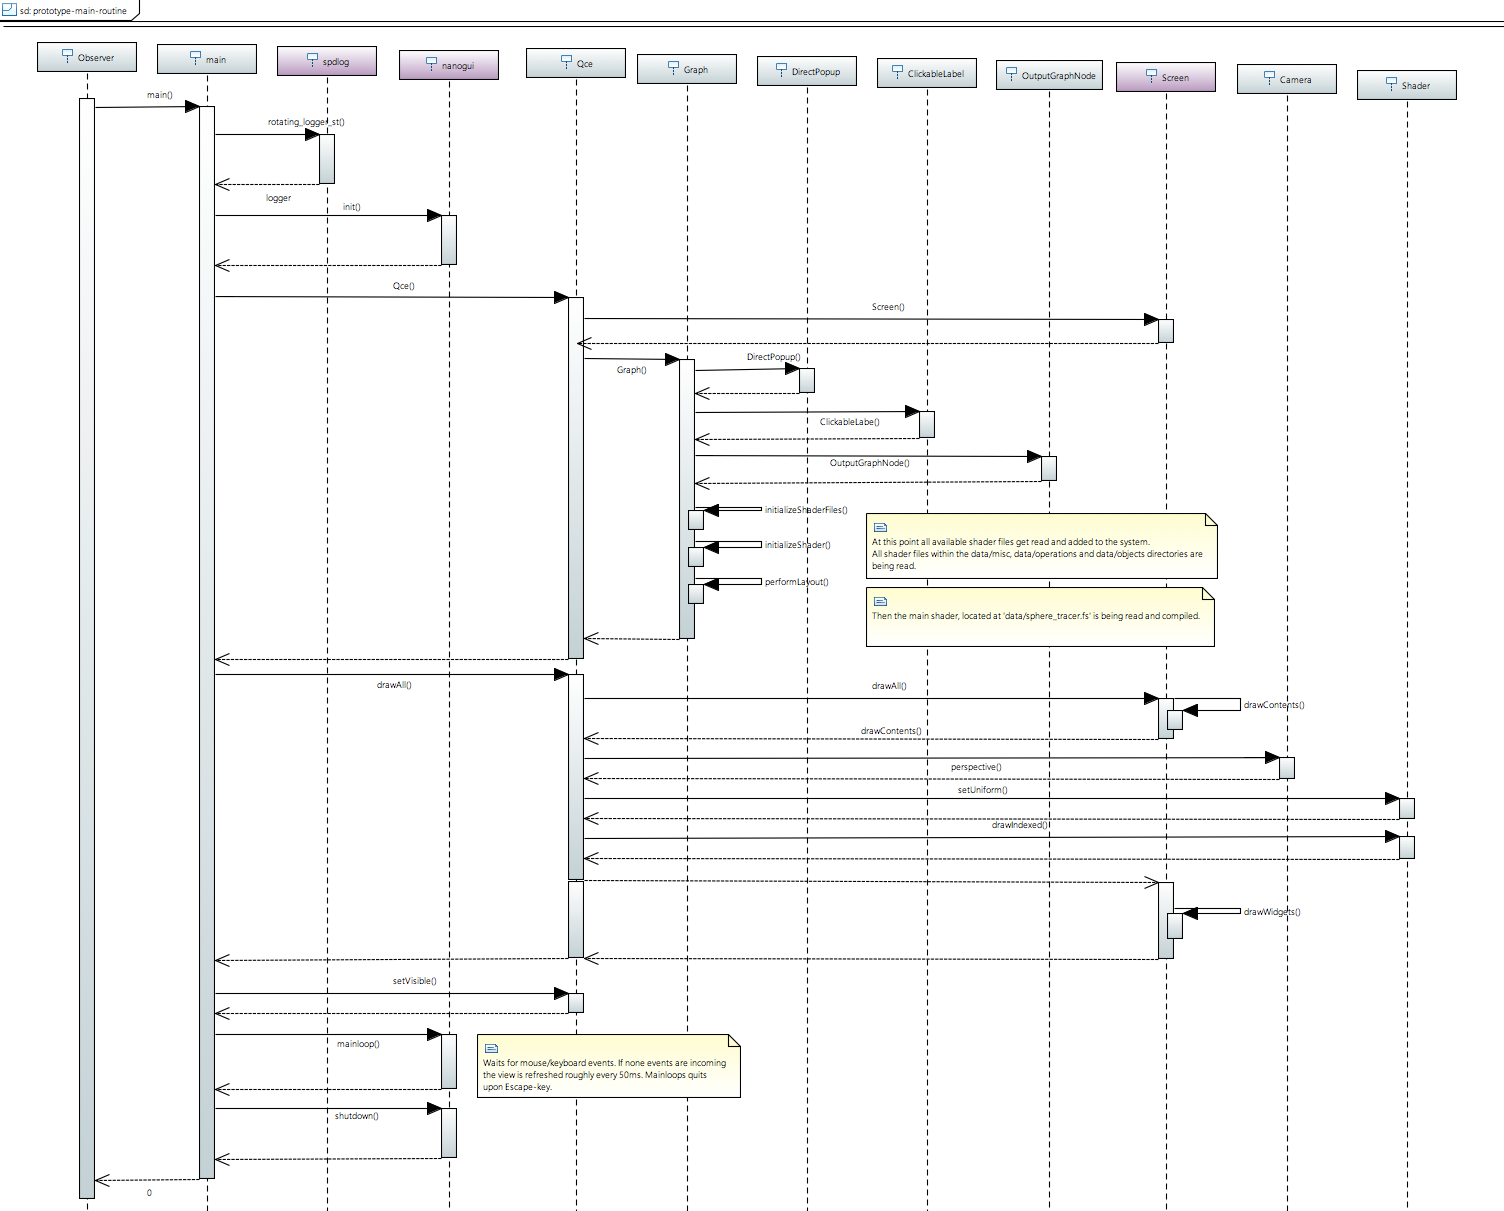
\includegraphics[width=0.9\textwidth]{img/prototype_sequence_diagram.png}
    \caption{Sequenz-Diagramm des Haupt-Ablaufes der
        Prototyp-Applikation\protect\footnotemark}\label{fig:sequence-diagram:prototype}
\end{figure}
\footnotetext{Eigene Darstellung mittels Papyrus.}


In Abbildung~\ref{fig:class-diagram:prototype} findet sich das Klassendiagramm
des Prototypen.  Blau-graue Elemente stellen dabei selbst entwickelte Pakete,
violette Elemente externe Pakete von Drittpersonen dar. Es wird bewusst
nicht das vollständige Klassendiagramm mit allen Elementen abgebildet, da dies
nach Meinung des Autors zu unübersichtlich würde. Die gesamte Struktur ist dem
Programmcode des Prototypen zu entnehmen, welcher dieser Projektarbeit
beiliegt.

\begin{figure}[H]
    \centering
    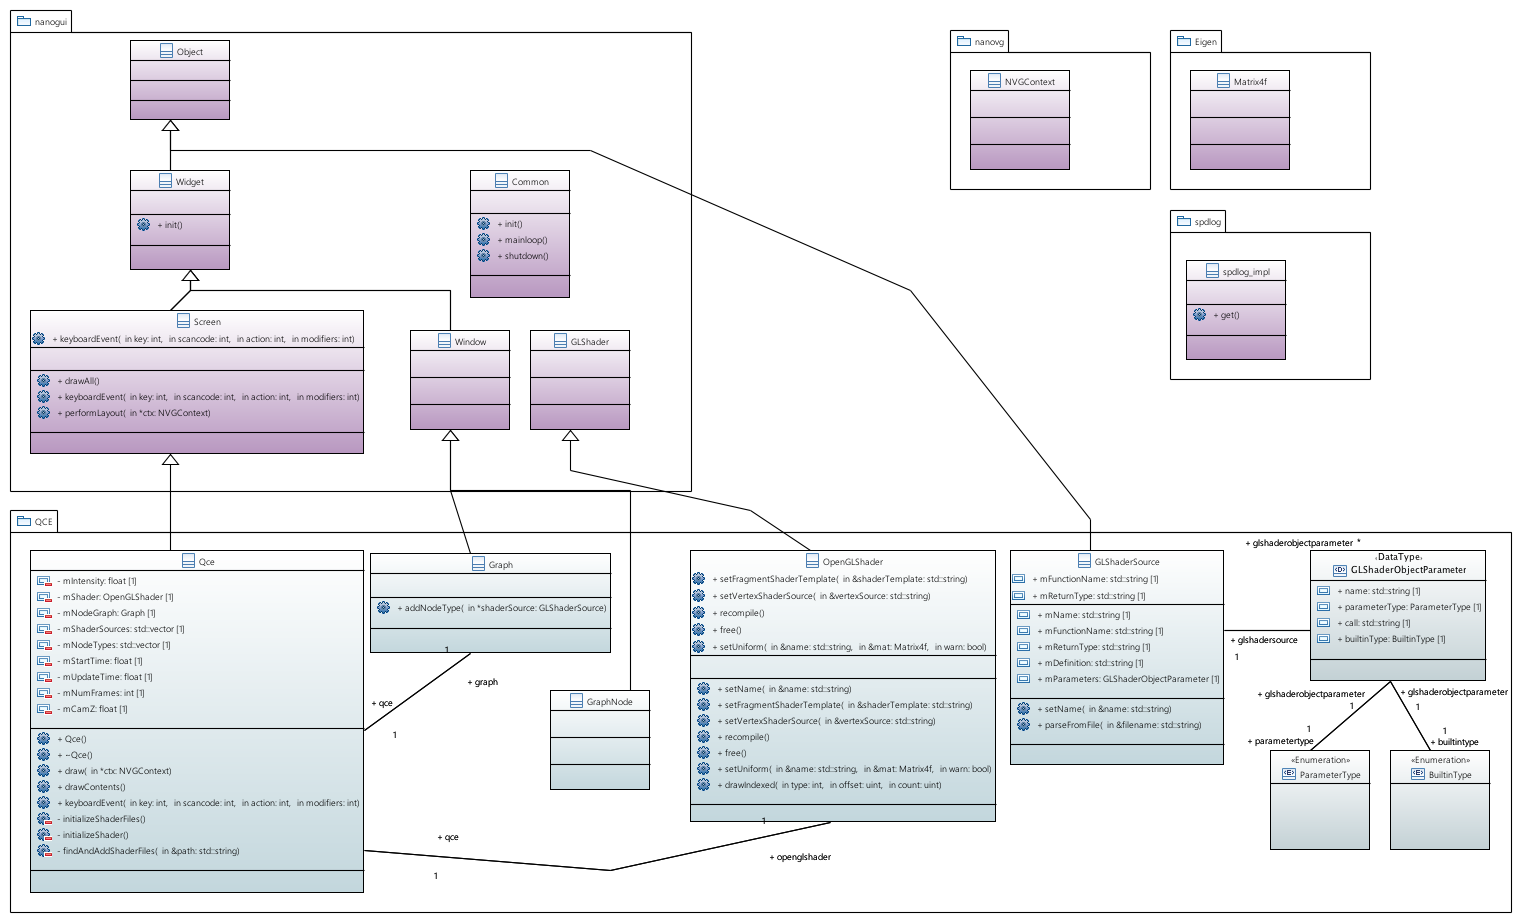
\includegraphics[width=0.9\textwidth]{img/prototype_class_diagram.png}
    \caption{Klassendiagramm der
        Prototyp-Applikation\protect\footnotemark}\label{fig:class-diagram:prototype}
\end{figure}
\footnotetext{Eigene Darstellung mittels Papyrus.}
